\documentclass[graphics]{beamer}

\usepackage{graphicx}
\usepackage{verbatim}
\usepackage{wrapfig}
\useoutertheme{shadow}
%\usecolortheme{orchid}
\usecolortheme{seahorse}


% math commands
\newcommand{\be}{\begin{eqnarray}}
\newcommand{\ee}{\end{eqnarray}}
\newcommand{\beq}{\begin{equation}}
\newcommand{\eeq}{\end{equation}}
\def\simless{\mathbin{\lower 3pt\hbox
      {$\rlap{\raise 5pt\hbox{$\char'074$}}\mathchar"7218$}}}
\def\simgreat{\mathbin{\lower 3pt\hbox
      {$\rlap{\raise 5pt\hbox{$\char'076$}}\mathchar"7218$}}} %> or of order

% variables

\def\toonscale{0.45}
\def\mboxy#1{\mbox{\small #1}}


\begin{comment}
\AtBeginSection[]{
  \frame{
    \frametitle{Outline}
    \tableofcontents[currentsection]
  }
}
\end{comment}

\title{Resolving the Hubble tension through diffraction of gravitational waves
}
%\subtitle{interim update}
\author[U. Pen]{Ue-Li Pen, Dylan Jow
}
\date{TPS2024 January 26, 2024}


\begin{document}

%\section*{Introduction}
\section{Lenses}

\begin{comment}
  \subsection{Outline}

  \frame{
    \frametitle{Outline}
    \tableofcontents
  }
\end{comment}

\frame{\maketitle}



  \frame{
    \frametitle{Diffractive/Effervescent Gravitational Wave Lensing}
\includegraphics[width=4.5in]{Figures/PTAGWLensing.pdf}

Jow+ in prep
  }


  \frame{
    \frametitle{Gravitational Waves -- Wave optics}
    \begin{itemize}
        \item Coherent, distant source of radiation
        \item Interference effects under multi-path propagation
        \item Kirchoff-Fresnel path integral
        \item semi-classical concepts: stationary phase, Eikonal limit
        \item Witten 2010: generalized by Picard-Lefschetz theory
        \item Morse index, effervescent/complex images: measure time delays in weak lensing
    \end{itemize}
  }


  \frame{
    \frametitle{Pulsar Timing Arrays (PTAs)}
    \begin{itemize}
      \item initial GW evidence in 2023 (nanoGrav++)
        \item currently from a few dozen nearby PSRs
        \item full map of galaxy with SKA, orders of magnitude
          improvement in sensitivity, resolution
        \item Precision distances with Scintillometry
        \item Coherent imaging GW telescope with arcsecond resolution
        \item no ``stochastic'' regime
        \item counterparts of supermassive BH binaries, precise redshifts
    \end{itemize}
  }

  \frame{
    \frametitle{Diffractive (effervascent) imaging}
    \begin{itemize}
        \item most galaxies too weak to form real gravitational lens images
        \item always form effervascent images through wave optics
        \item diffractive angle $\theta \sim \lambda/D$
        \item $\lambda \sim$ pc, $D\sim 500$pc $\longrightarrow \theta
          \sim 0.1^o$
        \item dominated by edge-on spirals!
    \end{itemize}
  }

  \frame{
    \frametitle{Time delay $H_0$}
    \begin{itemize}
        \item stack diffractive GW flux from all edge-on galaxies
        \item Shapiro delay neglible off-axis
        \item distance from angle-delay relation $\tau \sim \theta^2 L$.
    \end{itemize}
  }



  \frame{
\vspace{-0.25in}
    \frametitle{Optics: Geometric, Eikonal, Wave, P-L}
    \begin{itemize}
        \item Consider 1-D lens
        \item lensing potential $\Psi(\theta)$
        \item deflection $\Psi'$
        \item simplify for $D_{\rm ds}=\infty$
    \end{itemize}
\vspace{-0.5in}\hspace{2.5in}\includegraphics[width=1.5in]{Figures/lens.png}

  }




  \frame{
\vspace{-0.5in}
    \frametitle{Effervescent Images}
    \begin{itemize}
    \item consider ``rational lens'' potential $\psi(\theta)=\alpha/(1+\theta^2)$
    \item Geometric/eikonal images at $\psi'=\theta$
    \item 5 roots.  1 or 3 real roots, rest imaginary
    \item P-L: at most one imaginary image contributes!
    \item Resurgence theory to classify?
    \item Effervescent (imaginary) image can be brighter than unlensed real image
    \end{itemize}
  }


  \frame{
%\vspace{-0.5in}
    \frametitle{Rational 1-D lens}
\begin{center}
\includegraphics[width=3.1in]{Figures/theta-beta.eps}
\end{center}
  }

  
  \frame{
\vspace{-0.5in}
    \frametitle{Picard-Lefschetz Theory}
    \begin{itemize}
    \item descend integral along real line along Morse function Im(S)
    \item contour deforms into finite number of Thimbles of constant
      phase with maximum at saddle point (extrema $dS=0$)
    \item correctly identifies relevant saddle points
    \item resolves numerical challenges of oscillatory integral
    \item complex analysis works in multiple variables
    \item elevates concept of ``image'' deep into wave optics
    \item multiple public implementations (Feldbrugge+, Jow+)
    \end{itemize}
  }



  \frame{
\vspace{-0.5in}
    \frametitle{Picard-Lefschetz Theory}

\includegraphics[width=4.5in]{Figures/thimbles.png}

Feldbrugge+2019
  }





  \frame{
\vspace{-0.5in}
    \frametitle{Discussion}
    \begin{itemize}
    \item Eikonal effects applicable to compact radio sources,
      e.g. FRBs, pulsars
    \item full wave
effect dominates for long wavelengths as Fresnel scale is bigger then Einstein radius
    \item microlensing down to planet size
    \item gravitational waves:  LIGO, LISA, PTA
    \item with SKA PTA parameters and favourable source geometries, $H_0$
      measurement at 0.1\% possible.
    \end{itemize}
  }



  \frame{
%\vspace{-0.5in}
    \frametitle{Conclusions}
    \begin{itemize}
     \item wave optics changes nature of astrophysical observables: Coherent FRB/pulsar/GW      radiation one of the potentially most
      precise measurements in physics
      \item PTA weak diffractive lensing may give new tool for Hubble
        Constant tension
    \end{itemize}
  }

\end{document}
